\documentclass[12pt,letterpaper]{article}

\RequirePackage{xcolor}
\definecolor{tecAzul}{cmyk}{1,0.91,0.33,0.25} % según manual de imagen 2016
\definecolor{tecRojo}{cmyk}{0,0.9,0.86,0}     % según manual de imagen 2016
\definecolor{comando}{cmyk}{0,0.9,0.50,0} 
\renewcommand{\familydefault}{\sfdefault}

\usepackage[spanish,es-tabla]{babel}

\usepackage{titlesec}
\titleformat*{\section}%
{\normalfont\Large\bfseries\color{tecAzul}}
\titleformat*{\subsection}%
{\normalfont\large\bfseries\color{tecAzul}}


\usepackage[tmargin=2cm,bmargin=2cm,lmargin=2.5cm,rmargin=2.5cm]{geometry}
\usepackage{textpos}
\usepackage{tikz}
\usepackage{pgfplots}
\usepackage{pgf}
\usepackage{graphicx}
\usepackage{float}
\usepackage{array}
\usepackage{amssymb}
\usepackage{hyperref}
\usepackage{comment}
\usepackage{subfig}
\usepackage{listings}
\usepackage[margin=1cm]{caption}


%
% paragraph layout
%
\parindent0em                           % indentation width of first line
\parskip1.3ex                           % space between paragraphs


\title{Regresión polinomial y regresión ponderada localmente}

\newcommand{\EstudianteA}{Araya Fallas, Gerardo Enrique, gaf1@estudiantec.cr.}

\pgfplotsset{compat=1.17}

\begin{document}
	
\graphicspath{{./}{./fig/}}

%-------------------------- Title section -------------------------------------%

% kit logo
\begin{textblock}{10}[0,0](-0.5,0)
	\begin{flushleft}
		\large 
		Escuela de Ingeniería Electrónica \\
		Licenciatura en Ingeniería Electrónica \\
  		Profesor: Dr. Pablo Alvarado Moya\\
        EL 5857 Aprendizaje Automático\\
  		I Semestre 2024\\
	    \end{flushleft}
\end{textblock}

%Institute and Chair
\begin{textblock}{10}[0,0](2.9,-0.35)
	\begin{flushright}
		
\includegraphics[scale=0.8]{Firma_TEC-4.pdf}
	\end{flushright}
\end{textblock}

%% Title %%
\begin{center}
	\vspace{3.0cm}
	%{\Large\color{tecRojo} Tutorial de Proyecto }
	\par\vspace{.5cm}
	{\LARGE\bf\color{tecAzul}{Tarea 1: Gradientes, Matrices positivas definidas, Ecuaciones normales}
	\par\vspace{.3cm}
	{\large{\EstudianteA} 
	\vspace{0.3cm}}
\end{center}





\section{Introducción}
%------------------------------------------------------------------------------%
En esta tarea utilizaremos un escenario hipotético, en que queremos desarrollar un sensor eco-
nómico para medir profundidad en el océano. Como datos sintéticos de referencia (ground truth)
utilizaremos el perfil de la costa pacífica de Costa Rica tomado de este sitio.
El código base y los datos para esta tarea los encuentra en el repositorio de Github Classroom.
El sistema hipotético calcula datos de profundidad a partir de una red de sensores muy económicos,
que sin embargo, producen muestras en posiciones medidas con ruido en lugares arbitrarios, y con
valores ruidosos de profundidad.
Usted comparará los resultados de utilizar regresión polinomial y regresión ponderada localmente
(LWR o LOWESS) para procurar reconstruir de las muestras un mapa de profundidad aceptable.

%------------------------------------------------------------------------------%

%------------------------------------------------------------------------------%
\section{Objetivo}
1. Evaluar estrategias de regresión no lineal y determinar las ventajas y desventajas de cada
una.
2. Vectorizar procesos de cálculos complejos para aprovechar las capacidades de hardware mo-
derno y las implementaciones que ofrecen los sistemas para álgebra lineal.
3. Aplicar los conceptos teóricos desarrollados en las lecciones en la solución de un problema de
ingeniería.

\section{Marco Teórico}

\subsubsection{Propiedades de trazas y gradientes vistas en clase.}

\begin{figure}[H]
    \centering
    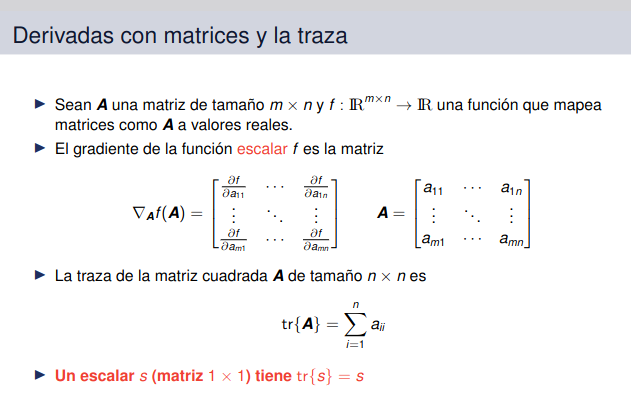
\includegraphics[scale=0.55]{A&A_GAF_HW01/fig/A&A_HW01_01.png}
    \caption{Propiedades de Derivadas de Matriz y Traza \cite{Teoría3.1_p35} } 
    \label{fig:MV4}
\end{figure}

\begin{figure}[H]
    \centering
    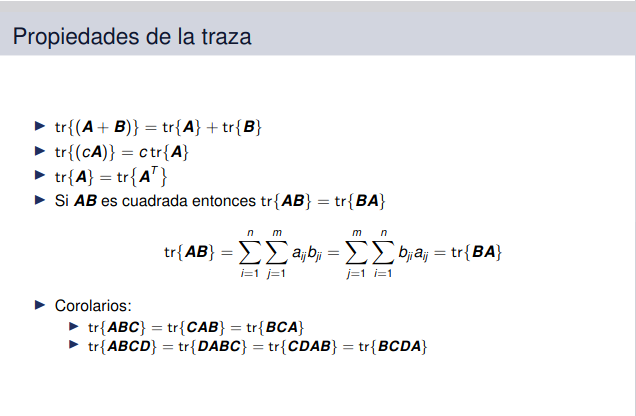
\includegraphics[scale=0.55]{A&A_GAF_HW01/fig/A&A_HW01_02.png}
    \caption{Propiedades de la Traza \cite{Teoría3.1_p35}   }
    \label{fig:MV4}
\end{figure}

\begin{figure}[H]
    \centering
    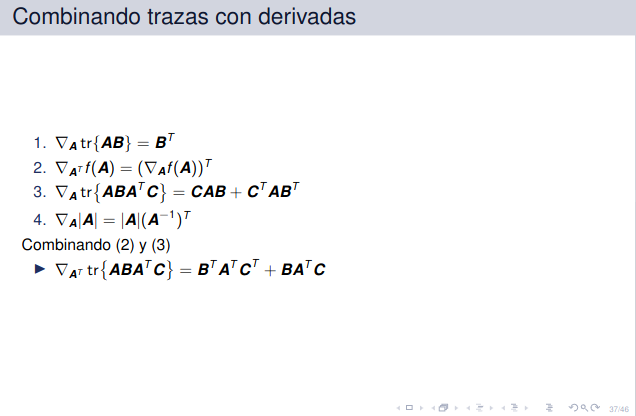
\includegraphics[scale=0.55]{A&A_GAF_HW01/fig/A&A_HW01_03.png}
    \caption{Combinado trazas con derivadas\cite{Teoría3.1_p35}   }
    \label{fig:MV4}
\end{figure}
\section{Gradientes} 
Sea la matriz A ∈ IRn×n simétrica, y sea el vector x ∈ IRn.
\\
1. Encuentre el gradiente ∇xf (x) para f (x) = 1 2 x⊤Ax + b⊤x utilizando las propiedades de trazas y gradientes vistas en clase.

 \begin{figure}[H]
    \centering
    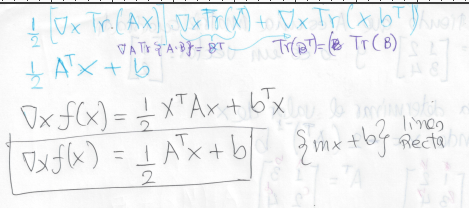
\includegraphics[scale=0.55]{A&A_GAF_HW01/fig/A&A_HW01_08.png}
    \caption{Gradiente de la función \cite{Mariano}   }
    \label{fig:MV4}
\end{figure}

La versión ampliada de la respuesta se encuentra en los anexos

\\
2. Realice una función en GNU/Octave que reciba una matriz A de tamaño 2 × 2 y un vector
b de dos dimensiones, y que grafique la superficie paraboloide tridimensional dada por
f (x) = 1
2x⊤Ax + b⊤x
en un rango de los componentes x1 y x2 de x = [x1, x2]⊤ también dado por el usuario.
Lo más relevante de este punto es que el código esté vectorizado, es decir, que se evite utilizar
ciclos for, y que todo se plantee en términos de sumas y productos de matrices y vectores
(incluyendo productos de Schur cuando sea necesario).
Algunas funciones que puede utilizar son, entre otras: sum, sumsq, vecnorm, dot, meshgrid,
surf, contour.

Para resolverlo se creo una función en Octave denominada funSupParTri(), a los cuales se le cargaron los valores de una matriz cuadrada denominada A= [1, 2, 3, 4], un vector b= [1; 2], y un rango entre [-10, 10]. el comando a ejecutar en OCTAVE es : funSupParTri([1, 2; 3, 4], [1; 2], [-10, 10])
Se analizo cada variable gráficamente, en una primera instancia los rangos bidimensionales generados y contenidos en x1 y X2


\begin{figure}[H]
    \centering
    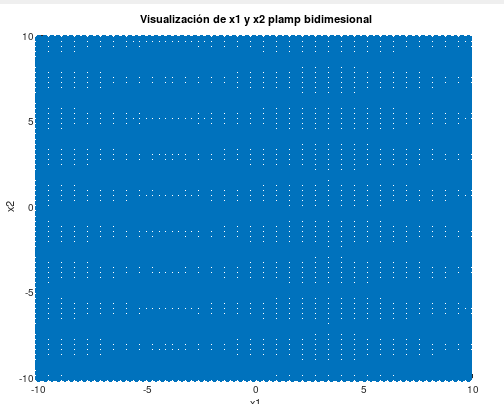
\includegraphics[scale=0.55]{A&A_GAF_HW01/fig/A&A_HW01_04.png}
    \caption{Gráfico bidimensional de x1 y x2   }
    \label{fig:MV4}
\end{figure}
Luego la visualización de las mismas variables pero tridimensional mente

\begin{figure}[H]
    \centering
    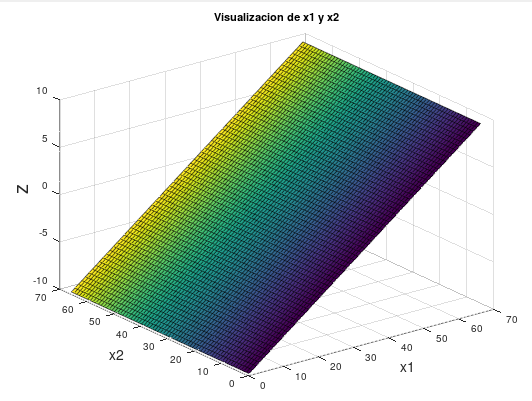
\includegraphics[scale=0.55]{A&A_GAF_HW01/fig/A&A_HW01_05.png}
    \caption{Función H optimizada \cite{Mariano}   }
    \label{fig:MV4}
\end{figure}
Las variables x1 y x2, se ordenaron en una sola matriz denominada X
\begin{figure}[H]
    \centering
    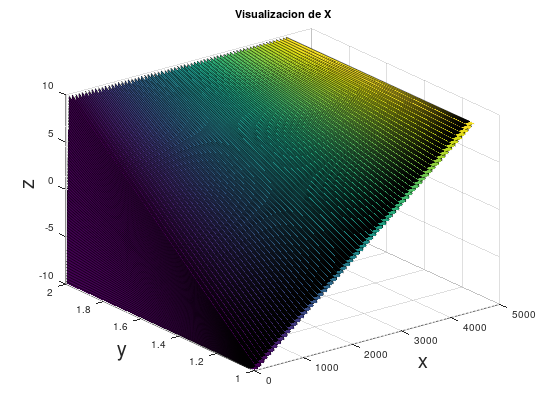
\includegraphics[scale=0.55]{A&A_GAF_HW01/fig/A&A_HW01_06.png}
    \caption{Ecuaciones canonicas diferenciales }   }
    \label{fig:MV4}
\end{figure}

Por ultimo se evalúa los valores de x en la función, dando como resultado la siguiente gráfica.

\begin{figure}[H]
    \centering
    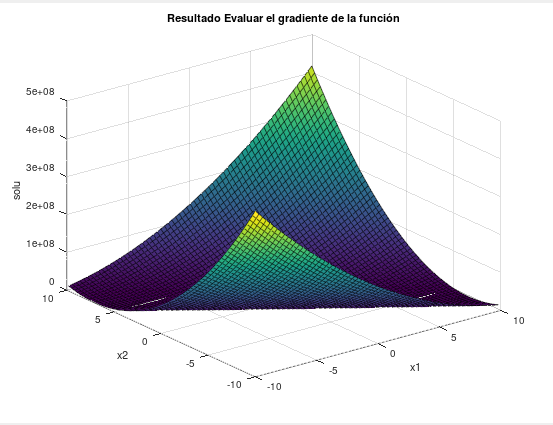
\includegraphics[scale=0.55]{A&A_GAF_HW01/fig/A&A_HW01_07.png}
    \caption{Resultado de evaluar el gradiente de la función} 
    \label{fig:MV4}
\end{figure}

3. Sabiendo que el mínimo se encuentra donde el gradiente de la función es cero, encuentre
dónde está el mínimo de la función.

\begin{figure}[H]
    \centering
    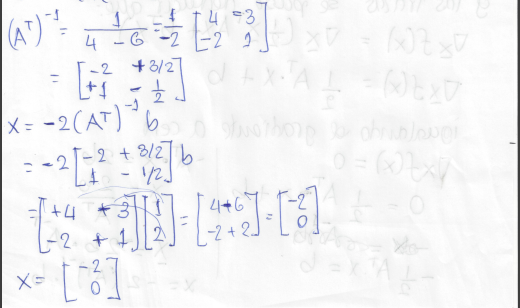
\includegraphics[scale=0.55]{A&A_GAF_HW01/fig/A6A_HW01_09.png}
    \caption{Diagrama de bloques. Algoritmo de optimización }}   \label{fig:MV4}
\end{figure}

\\
la solucion ampliada de evaluar el gradiente en cero se encuentra en el anexo
\
\
4. Use su función para mostrar tres casos de paraboloides: (10 pts)
Elija b distinto de cero y los rangos de x, de modo que el mínimo del paraboloide sea visible.


4.1. Matriz A igual a la matriz identidad escalada cI, evaluada con la siguiente función: function  FSPT_P401(M22, V02, Rangos, Const)

\begin{figure}[H]
    \centering
    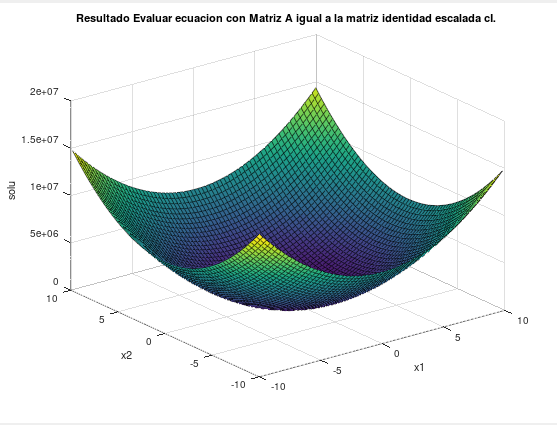
\includegraphics[scale=0.55]{A&A_HW01_10.png}
    \caption{Diagrama de bloques. Algoritmo de optimización }}   \label{fig:MV4}
\end{figure}


4.2. Matriz diagonal pero con los dos elementos de la diagonal distintos.

Evaluada con la siguiente función: FSPT_P402(M22, V02, Rangos, Const)

\begin{figure}[H]
    \centering
    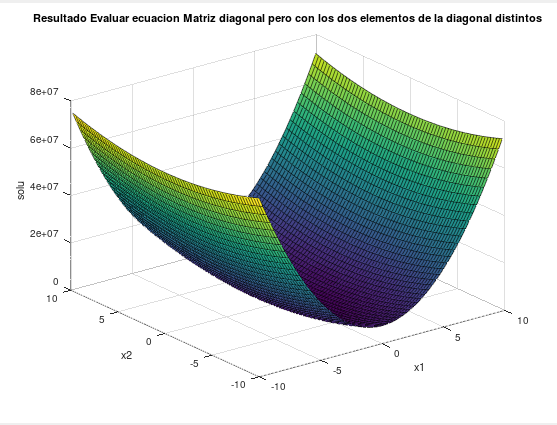
\includegraphics[scale=0.55]{A&A_GAF_HW01/A&A_HW01_11.png}
    \caption{Diagrama de bloques. Algoritmo de optimización }}   \label{fig:MV4}
\end{figure}


4.3. Matriz simétrica no diagonal, que debe ser positiva definida.

\begin{figure}[H]
    \centering
    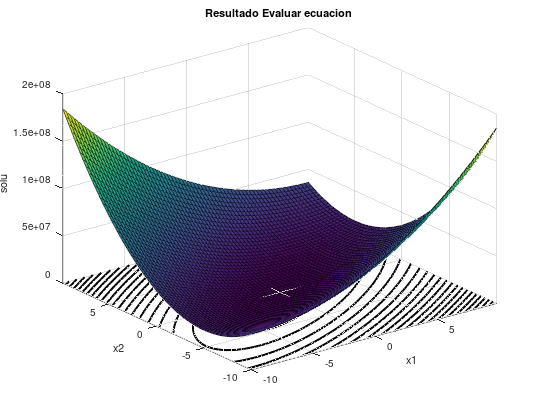
\includegraphics[scale=0.55]{A&A_GAF_HW01/A&A_HW01_12.png}
    \caption{Diagrama de bloques. Algoritmo de optimización }}   \label{fig:MV4}
\end{figure}

5. Utilice ahora la función quiver para mostrar además el gradiente de la función paraboloide
del punto 4.3. 
\begin{figure}[H]
    \centering
    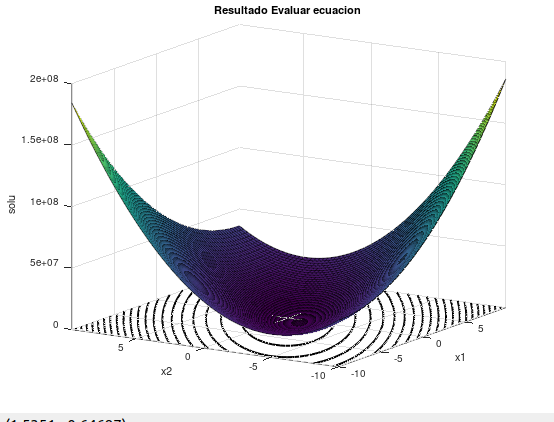
\includegraphics[scale=0.55]{A&A_GAF_HW01/A&A_HW01_13.png}
    \caption{Diagrama de bloques. Algoritmo de optimización }}   \label{fig:MV4}
\end{figure}

%------------------------------------------------------------------------------%







%------------------------------------------------------------------------------%


\
\end{document}









